\section{Introduction}

The novel coronavirus, SARS-CoV-2, originated in Wuhan, China in late 2019 and rapidly spread around the world \citep{chen20,wu20}. This virus causes the Covid-19 disease which can lead to severe illness needing long hospitalization \citep{sun20,goyal20,jiang20}, but at the same time a significant fraction of those who contract the virus experience an asymptomatic Covid-19 disease \citep{he20}. It is still not entirely clear who is at risk for developing severe disease, although correlations of disease severity with levels of vitamin D \citep{ilie20}, levels of various immune components \citep{liu20imm,liu20imm2,zhang20imm,yang20imm}, and age \citep{borghesi20,zhang20imm} have been noted. There has also been investigation of the possibility of disease severity being linked to initial viral inoculum \citep{little20, guallar20, ghandi20}.

The major route of transmission for SARS-CoV-2 is airborne droplets \citep{morawska20}. One study indicates that sneezing and coughing creates a turbulent gas cloud that can cause viral-laden droplets to spread up to 27 feet (\numrange[range-phrase = --]{7}{8}\si{\meter}) \citep{bourouiba20}, and allows the virus to get into the ventilation system of a building. A review of literature on droplet and airborne viral spread concludes that 8 of 10 studies showed that droplets spread further than the 6 foot \citep{bahl20} social distancing recommendation. While personal protective equipment is helpful in reducing the ability of virus to enter the respiratory tract, it is not perfect \citep{mittal20}. All of these factors lead to exposures to vastly different quantities of virus when people are going about their daily activities. Thus it is important to understand whether different initial inocula lead to different viral dynamics in patients. 

There is some evidence from other respiratory viruses that the size of the initial inoculum could play a role in the severity of the illness. An influenza epidemiological modeling study suggests that a higher initial dose can lead to a higher mortality rate \citep{paulo10}. This is corroborated by an influenza in-host modeling study that also finds a correlation between the initial viral dose and survival rate \citep{price15}. Other modeling studies have found dependence of other measures of infection severity on initial dose for influenza \citep{moore20}, respiratory syncytial virus \citep{wethington19}, adenovirus \citep{li14}, and porcine reproductive and respiratory virus \citep{go19}. There are also experimental studies that find a link between dose and infection severity. Experiments using influenza have found inoculum dose dependence of total number of infected cells and area under the curve \citep{manicassamy10}, peak viral titer \citep{ginsberg52,iida63,ottolini05}, viral growth rate \citep{ginsberg52}, and time of viral peak \citep{iida63,ginsberg52}. Experiments with other viruses, such as adenovirus \citep{prince93}, and parainfluenza \citep{ottolini96}, have also shown correlations between initial inoculum and various measures of disease severity. If SARS-CoV-2 shows a similar pattern, initial inoculum should be considered as a possible contributor to infection severity and adverse outcomes.

\subsection{Mathematical model}

We use an ABM to model transitions of cells as they go through the infection cycle. We use a hexagonal grid and simulate 10$^6$ cells in a circular dish to mimic an in vitro system. Cells begin as healthy target cells that can be infected by viruses that are sitting above them. Once infected, the cells move into an eclipse phase where they are not yet actively producing virus. The cells remain in the eclipse phase for a time chosen from an Erlang distribution with mean time $\tau_E$ and shape parameter $n_E$. The cells then pass into the infectious phase, where they are actively producing virus, for a time chosen from an Erlang distribution with mean time $\tau_I$ and shape $n_I$, after which time the cells die and no longer participate in the infection. Erlang distributions are used for both transitions based on experiments that show the time spent in the eclipse phase and the time spent in the infectious phase are best described by Erlang distributions \citep{kakizoe15, beauchemin17}, at least for SHIV. While SHIV is a different virus, it is the only virus for which these distributions have been measured directly. Influenza, another respiratory virus, has also been shown to need non-exponential transition distributions \citep{holder11autoimm, holder11}. 

Viral dynamics are described by the PDM as virus diffuses over the layer of cells,
\begin{equation}
\frac{\partial V}{\partial t} = D\nabla^2V+p-cV,
\end{equation}
where $D$ is the diffusion coefficient, and $c$ is the viral decay rate. Virus is produced by infectious cells at rate $p$ and is assumed to be released directly above each infected cell. The amount of virus above any cell determines the probability that the cell will be infected, $P_\mathrm{inf}=\beta V$, where $P_\mathrm{inf}$ is the probability per unit time, and $\beta$ is the infection rate. A more detailed description of the model is given in the supplementary material and the simulation code is available on https://github.com/BaylorFain/Covid19-Code.

Parameter values that describe SARS-CoV-2 are taken from a variety of sources and are given in Table \ref{params}. The majority of the parameters are taken from \citep{pinky20}, where an ordinary differential equation model of coronavirus infection was fit to viral titer data from a single patient. Note that the parameters $\beta$ and $p$ are scaled to account for the different numbers of cells (10$^6$ here and 1 in \citep{pinky20}) in the two systems as well as converting viral concentration to individual virions (see \citep{handel07,perelson12,dobrovolny17} for detailed discussions on converting from concentration to virions). The shape parameters are based on values derived from influenza infections \citep{pinilla12}, since the Erlang distribution has not yet been used for SARS-CoV-2. The diffusion coefficient was calculated using the Stokes-Einstein equation \citep{cush97}. 
\begin{table}
\centering
\caption{Parameter values to simulate SARS-CoV-2 infection with the ABM/PDM model.\label{params}}
\resizebox{\textwidth}{!}{%
\begin{tabular}{llc}
\hline
Parameter & Meaning & Value \\
\hline
$\beta^a$ & Infection rate & $\SI{84.0}{\per\hour}$ \\
$\tau_E^b$ & Mean eclipse duration & \SI{5.88}{\hour} \\
$n_E^c$ & Eclipse shape parameter & 30 \\
$\tau_I^b$ & Mean infectious lifespan & \SI{0.624}{\hour} \\
$n_I^c$ & Infectious shape parameter & 100 \\
$p^a$ & Viral production rate & $\SI{19900}{\per\hour}$ \\
$c^b$ & Viral clearance rate & \SI{0.00490}{\per\hour} \\
$D^d$ & Diffusion coefficient & $\SI{4.80e-12}{\meter^2\per\second}$ \\
\hline
\multicolumn{2}{l}{$^a$Parameters taken from \citep{pinky20}, but scaled.}\\
\multicolumn{2}{l}{$^b$Parameters taken from \citep{pinky20}.}\\
\multicolumn{2}{l}{$^c$Parameters taken from \citep{pinilla12}.}\\
\multicolumn{2}{l}{$^d$Parameter calculated from Stokes-Einstein equation.}
\end{tabular}}
\end{table}

\subsection{Measurements}

We simulate SARS-CoV-2 infections starting with different multiplicity of infection (MOI) where the MOI value defines the initial number of infected cells. The ABM/PDM model is implemented in Compute Unified Device Architecture (CUDA) and run on NVIDIA graphics processing units. We perform 100 simulated infections for each MOI and measure the following features of the viral titer curve (Fig.\ \ref{measurements}): 
\begin{itemize}
\item \textbf{peak viral load:} The maximum amount of virus is commonly used as an indicator of the transmissibility of an infection \citep{handel09}. 
\item \textbf{time of viral peak:} This is the time between the start of the infection and the peak of the virus and can give an indication of how quickly the virus is replicating.
\item \textbf{viral upslope:} Viral upslope is the exponential growth rate of the viral titer before the peak is reached and is another indication of how quickly the virus is spreading from cell to cell. 
\item \textbf{area under the curve (AUC):} AUC is often used to assess the severity of an infection \citep{hayden00, barroso05}.
\item \textbf{infection duration:} The infection duration is indicative of how long an infected patient might test positive for presence of the virus. Note that the threshold used here is 10$^7$ virions based on a 10$^2$ RNA copies/ml detection threshold for the experimental data \citep{goncalves20} that is converted to individual virions.
\end{itemize}
\begin{figure}[!h]

\begin{center}
\resizebox{0.6\textwidth}{!}{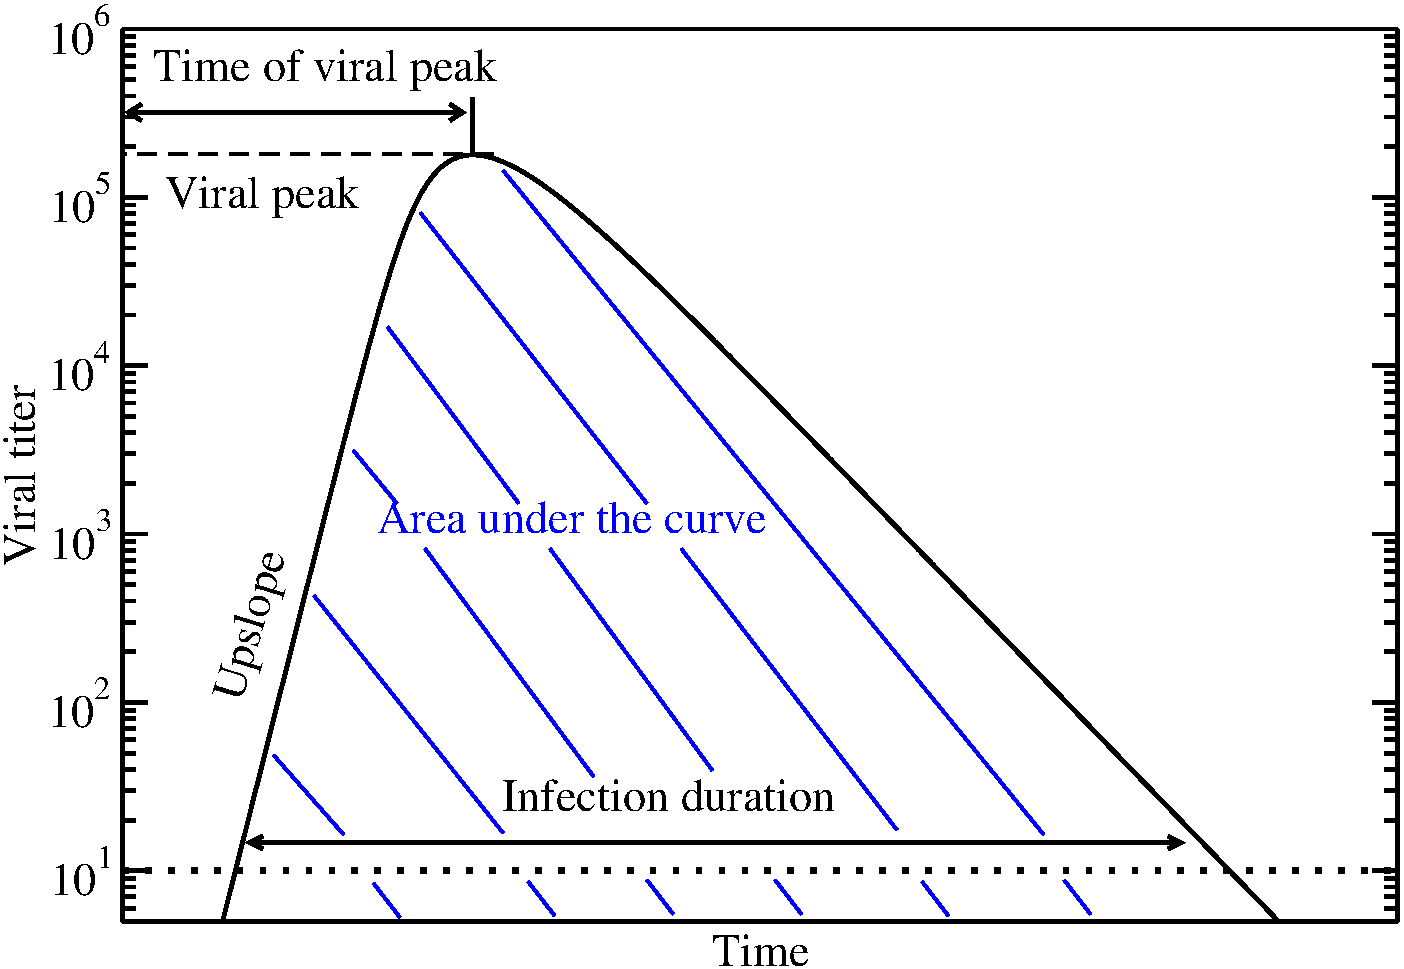
\includegraphics{Figures/measurements}}
\caption{Characteristics of the viral titer curve that are used to assess severity of the infection.\label{measurements}}
\end{center}
\end{figure} 


\section{Results}

Fig.\ \ref{curves} shows the viral titer curves for different MOI of SARS-CoV-2, where the darker line for each color shows the curve of median values and the lighter colored lines are the 100 individual simulations. Note that for most MOI, there is very little variation between simulations once the viral titer is large. The exception is the lowest MOI of 10$^{-5}$ where there is more variation in the exact trajectory of the viral load. We see some obvious shifts in the viral titer curve as the MOI increases. For high MOI, the viral titer curve reaches its peak very quickly, with lower MOIs moving the peak farther out in time. The peak also becomes broader and lower as the MOI becomes lower, suggesting longer infection durations, but with lower viral loads.
\begin{figure}[!h]
\begin{center}
\resizebox{0.6\textwidth}{!}{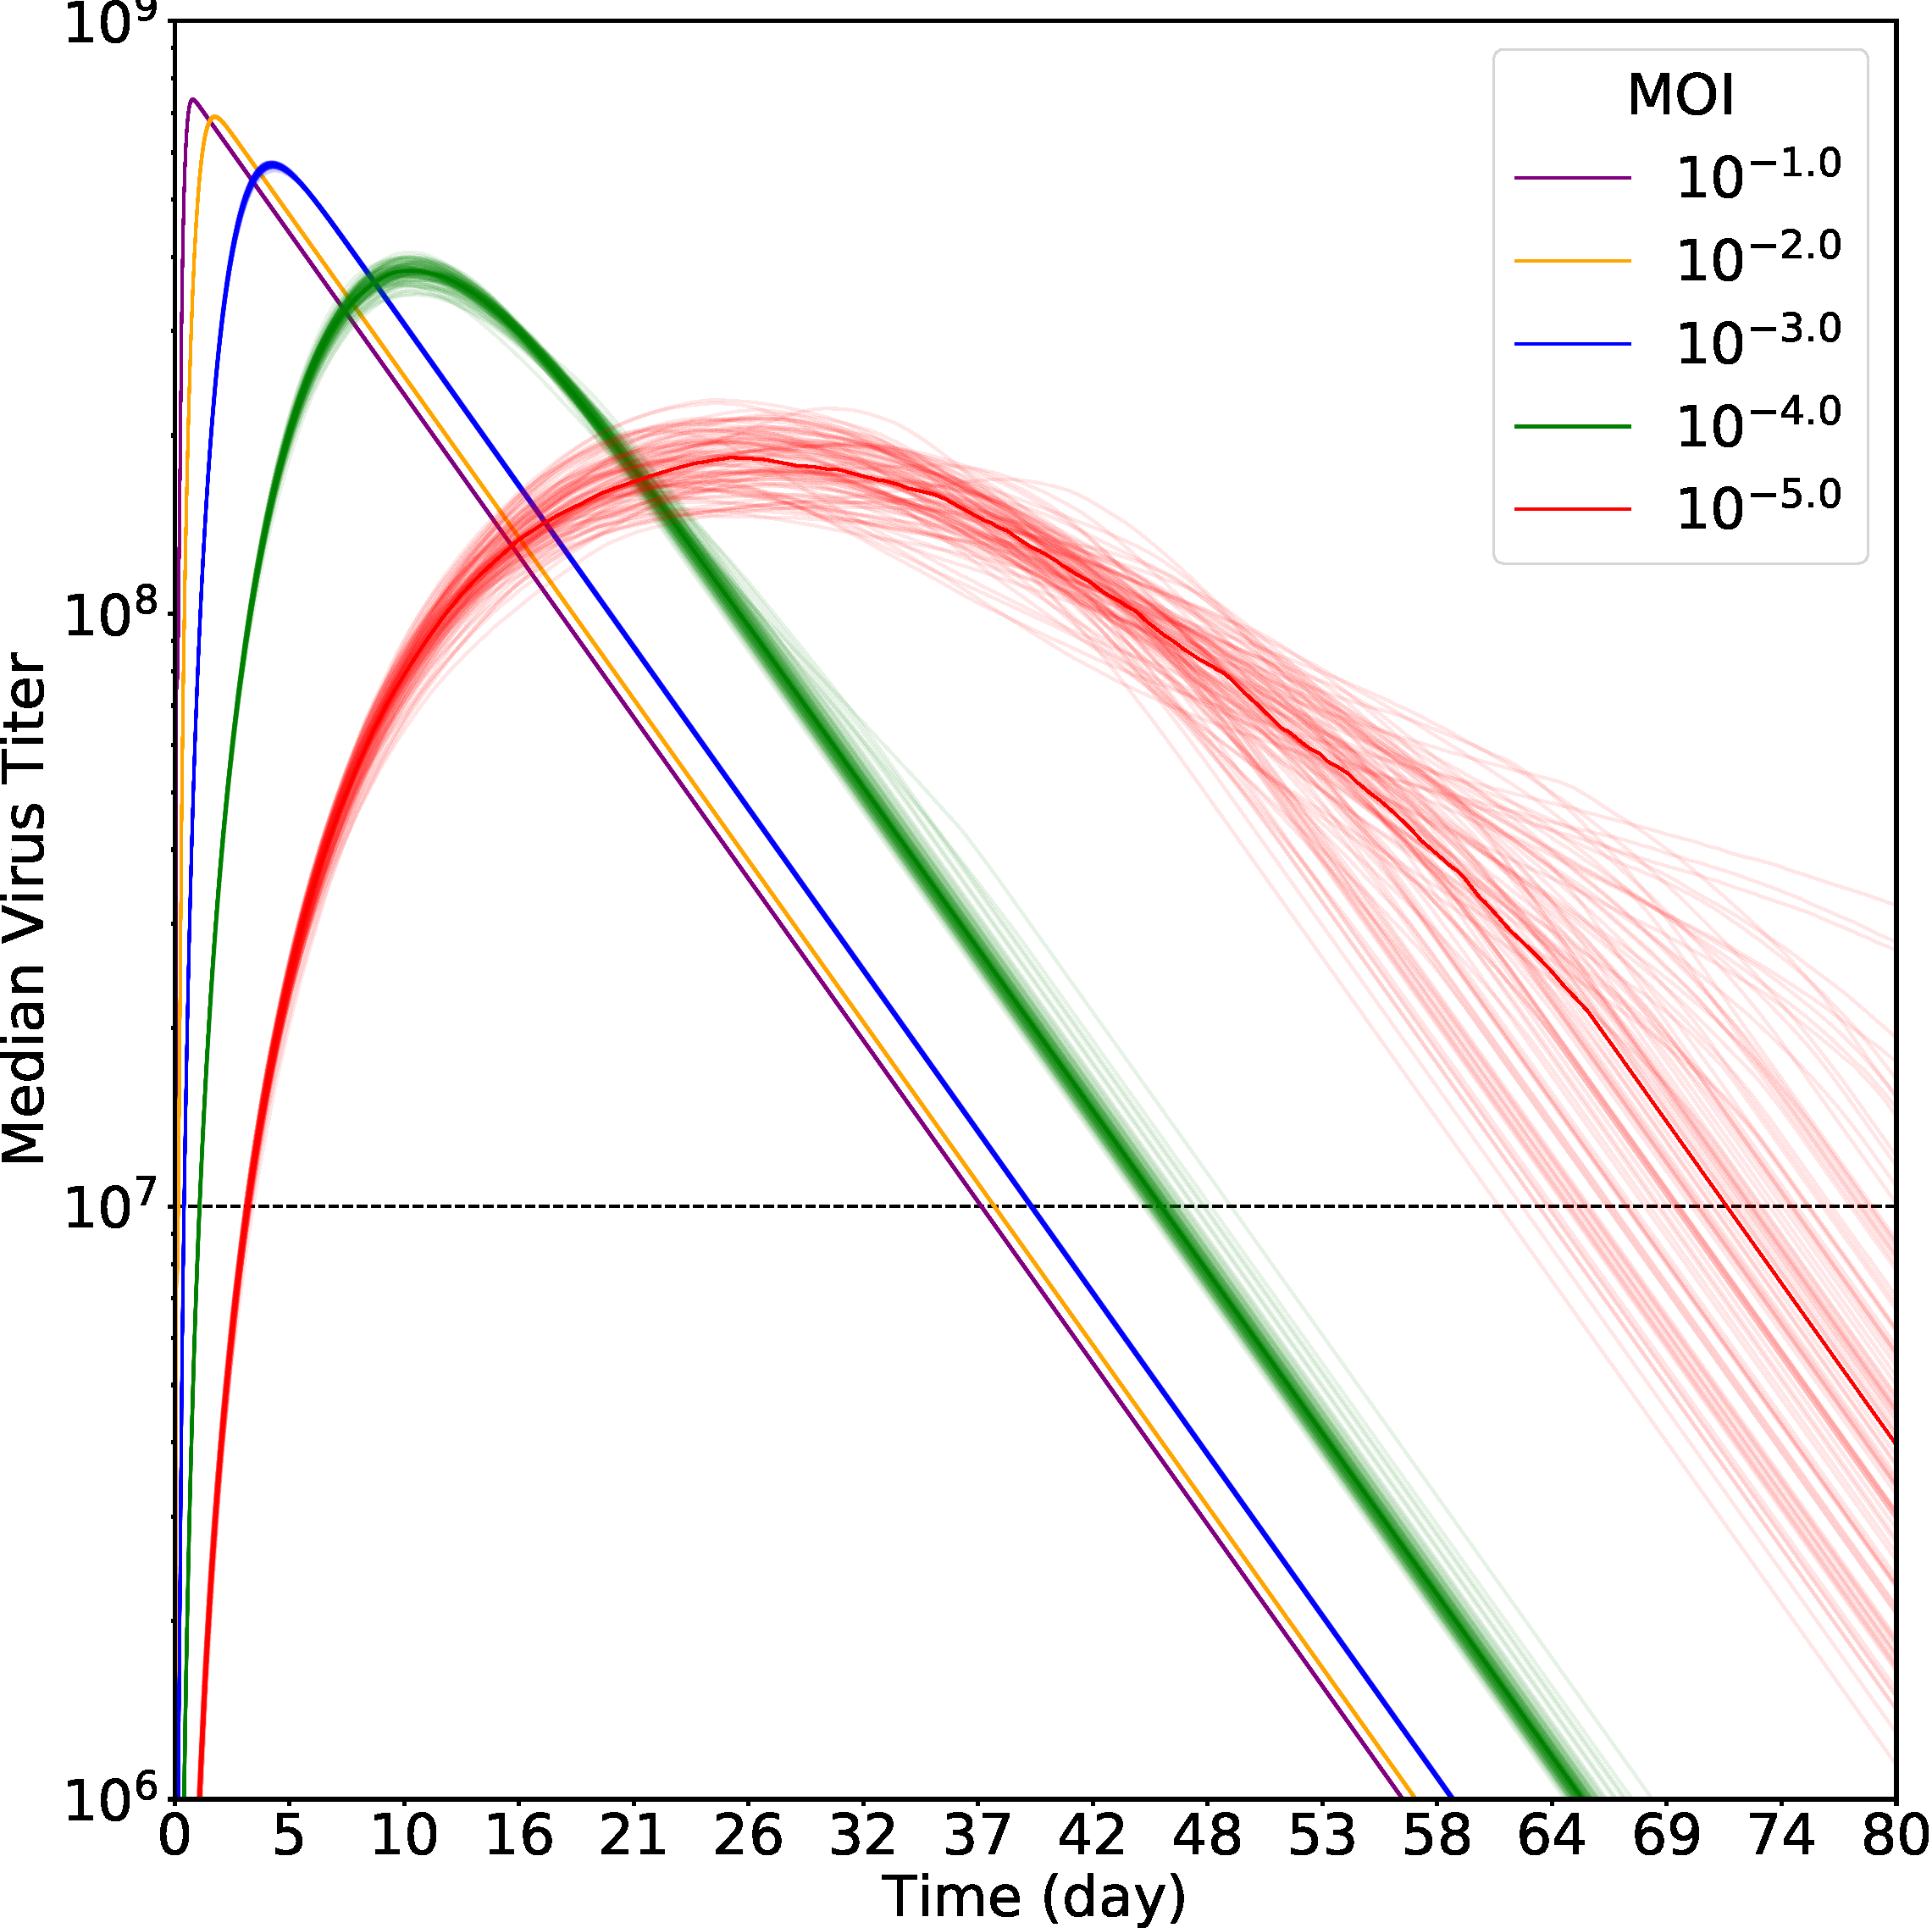
\includegraphics{Figures/Covid_AllOnOne_Median_VirusVsTime}}
\caption{Viral loads for infections initiated with different MOI. Dark lines of each color indicate the viral load curve using the median of 100 simulations, while the lighter colored lines show the viral load kinetics for each individual simulation. The dashed line indicates the threshold of detection used to calculate infection duration. \label{curves}}
\end{center}
\end{figure}

For a more quantitative assessment, we measure the characteristics described in Methods. The results are shown in Fig.\ \ref{results}, which shows peak viral load (top left), time of viral peak (top right), viral upslope (center left), AUC (center right), and infection duration (bottom) as functions of the MOI. The peak viral load increases with increasing initial inoculum, but it appears to reach a plateau as we near an MOI of 1. The time of peak, on the other hand, decreases with increasing initial inoculum, reaching a fixed small value at high MOI. There are real plateaus here since each cell will produce an average of $p\tau_I$ viral particles. At an MOI of 1, all cells are initially infected and will start producing virus at about the same time, meaning that all that virus is released almost simultaneously and there is no second cycle of infection. At slightly lower MOIs, most cells are initially infected, but some cells will be infected in a second or third cycle of infection, reducing the large burst of virus at one time, which causes a delay, reduction, and broadening in the peak. The upslope, or growth rate, of the viral titer curve increases as the MOI increases. This is also driven by the larger amount of virus being produced in the first cycle of infection as the MOI increases. Finally, the AUC and infection duration both decrease as the initial inoculum increases.  
\begin{figure}[!h]
\begin{center}
%\resizebox{0.48\textwidth}{!}{\includegraphics{Figures/CovidApectGraphs/PeakViralTitter}}
%\resizebox{0.48\textwidth}{!}{\includegraphics{Figures/CovidApectGraphs/TimeofPeakViralTitter}}
%\resizebox{0.48\textwidth}{!}{\includegraphics{Figures/CovidApectGraphs/New_UpSlope}}
%\resizebox{0.48\textwidth}{!}{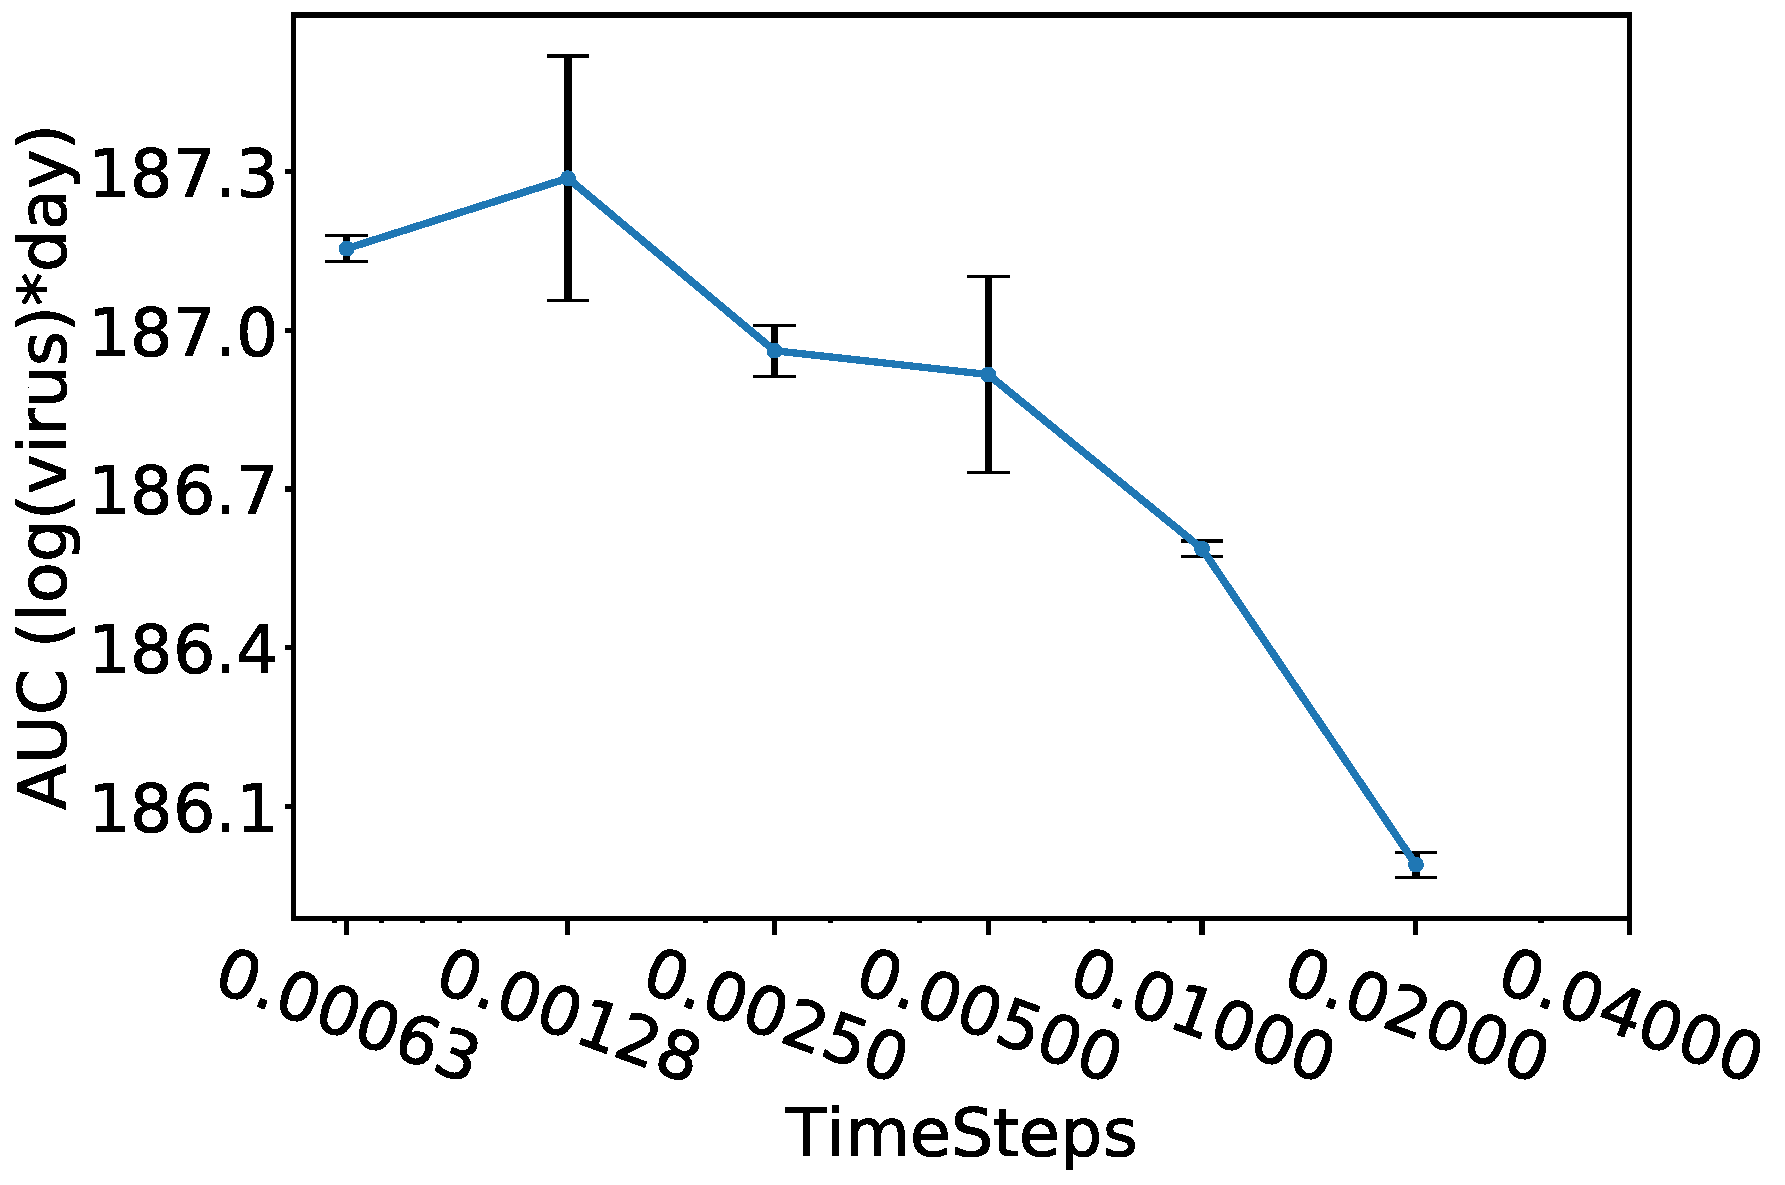
\includegraphics{Figures/CovidApectGraphs/AUC}}
%\resizebox{0.48\textwidth}{!}{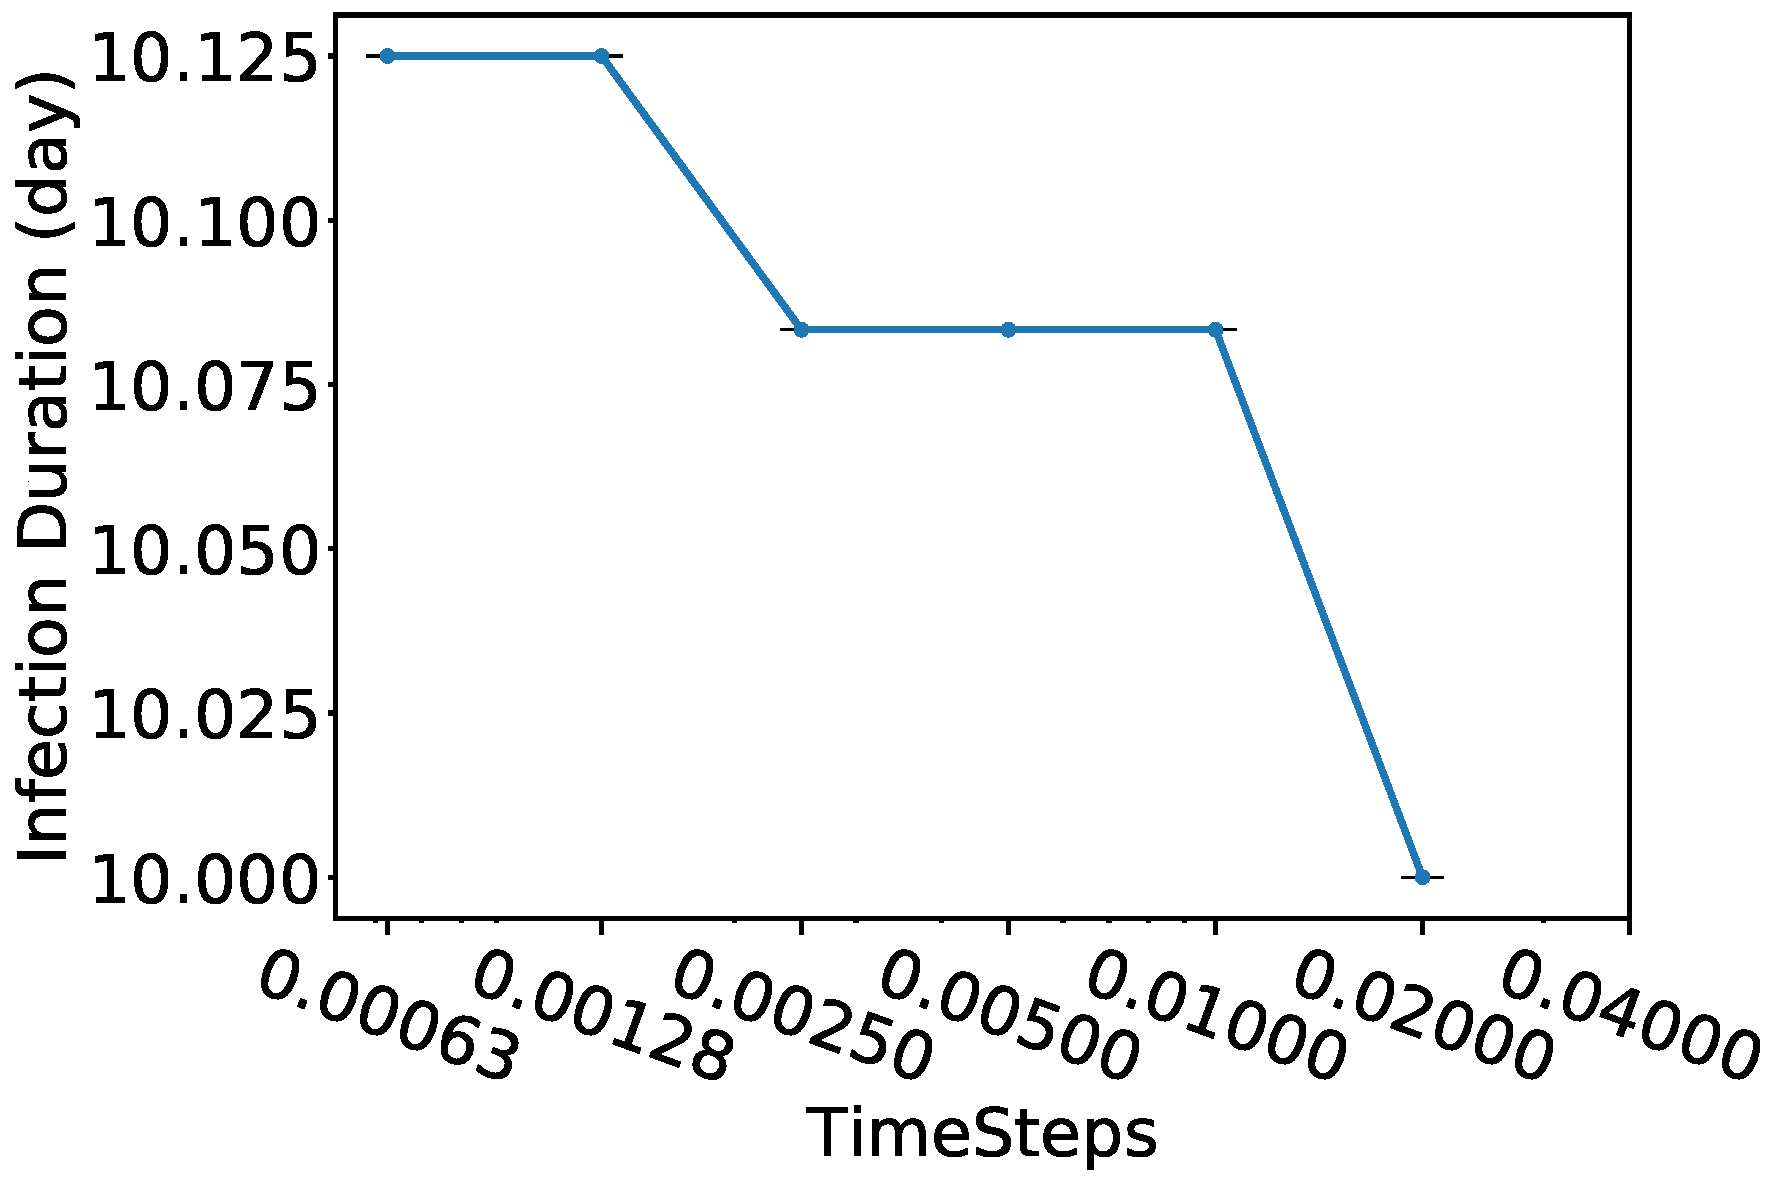
\includegraphics{Figures/CovidApectGraphs/InfectionDuration}}
\caption{Effect of initial inoculum on viral titer characteristics. The graphs show peak viral load (top left), time of viral peak (top right), viral upslope (center left), AUC (center right), and infection duration (bottom) as functions of MOI. \label{results}}
\end{center}
\end{figure}

%%%%%%%%%%%%%%%%%%%%%%%%%%%%%%%%%%%%%%%%%%
\section{Discussion}

Our study finds that initial viral inoculum does alter the viral time course by increasing the peak viral load, moving the peak earlier, increasing the viral upslope, and decreasing both AUC and infection duration, as the initial inoculum increases. 


